%!TEX root = MagicSquare.tex

In this section, we introduce our main robust self-testing theorem for linear constraint system games with solution groups of a certain form. In \S \ref{subsection:exact-self-testing}, to ease understanding, we start by stating and proving an exact version of the theorem. In \S \ref{subsection:state-dependent-distance} through \S \ref{subsection:quant-stabilizer-state-bounds}, we introduce the necessary tools to prove an approximate version of the self-testing theorem. \S \ref{subsection:state-dependent-distance} introduces the state-dependent distance and some of its properties. \S \ref{subsection:stability-lemma} proves a stability lemma for representations of finite groups, which allows us to deduce that the action of a strategy winning with high probability is close to the action of a representation of the solution group.  \S \ref{subsection:quant-van-kampen} presents a quantitative version of the van Kampen Lemma from Section \S \ref{subsection:van-kampen-diagrams}, which is key in bounding the robustness of the main theorem. \S \ref{subsection:quant-stabilizer-state-bounds} shows that if a joint state is approximately stabilized by the action of the Pauli group on two tensor factors, then it is close to the maximally entangled state on the two tensor factors. In \S \ref{subsection:robust-self-testing} we combine these tools to prove our robust self-testing theorem. 
 
\subsection{Exact self-testing}
\label{subsection:exact-self-testing}

Throughout, let $\LCS(\mathbf H, l, \Z_d), \mathbf H = (V,E,H)$ be an LCS game with solution group $\G$.

\begin{thm}[Rigid self-testing of observables]\label{thm:rigid-self-testing-observables}
Suppose $\G$ is finite and all of its irreducible representations with $J\mapsto \w_d I$ are equivalent to a fixed irrep $\s:\G\to U(\C^d)$. Suppose $\set{A_e^{(v)}}, \set{B_e}, \rho\in \m L(\m H_A\otimes \m H_B)$ is a perfect strategy presented via observables for the game. 
Then there are local isometries $V_A, V_B$ such that
	\begin{itemize}
		\item for all $e,v$, $V_AA_e^{(v)}V_A^\dagger = \s(e)\otimes I \oplus \hat A^{(v)}_e$, where $\hat A^{(v)}_e V_A\rho V_A^\dagger = 0$, and 
		\item for all $e$ $V_BB_eV_B^\dagger =\bar{\s(e)}\otimes I \oplus \hat B_e$, where $\hat B_e V_B\rho V_B^\dagger = 0$.
	\end{itemize}
\end{thm}
Awkwardly, we must pick a basis to take the complex conjugate in. Fortunately, we only care about our operators up to isometry. So to make sense of the theorem statement, we pick the basis for complex conjugation first, and then the isometry $V_B$ depends on this choice.
 We break the proof into two lemmas.
\begin{lemma}\label{lem:unique-operator-solution}
	Suppose $\G$ is finite and all of its irreducible representations with $J\mapsto \w_dI$ are equivalent to a fixed irrep $\s:\G\to U(\C^d)$. Then every operator solution is equivalent to $\s\otimes I$ and every conjugate operator solution is equivalent to $\bar{\s}\otimes I$, where the complex conjugate can be taken in any basis. 
\end{lemma}

\begin{lemma}[Adapted from Lemma 8, \cite{cleve2016perfect}]\label{lemma:CLS}
Suppose $\set{A_e^{(v)}}, \set{B_e}, \rho\in \m L(\m H_A\otimes \m H_B)$ is a perfect strategy presented via observables for the game. 
	Then, there are orthogonal projections $P_A, P_B$ such that 
	\begin{enumerate}
	\item $(P_A\otimes P_B)\rho(P_A\otimes P_B) = \rho$;
	\item for each $e$, $P_AA_e^{(v)}P_A = P_AA_e^{(v')}P_A$, provided that $H(v,e) \neq 0 \neq H(v',e)$ (we now write $P_AA_eP_A$ without ambiguity);
	\item the map $\s_A:\G\to \ran P_A$ generated by $e\mapsto P_AA_eP_A$ (and $j \mapsto \w_dI$) is an operator solution;
	\item the map $\s_B:\G\to \ran P_B$ generated by $e\mapsto P_BB_eP_B$ (and $j \mapsto \bar{\w_d}I$) is a conjugate operator solution.
	\end{enumerate}
\end{lemma}

\begin{proof}[Proof of Theorem \ref{thm:rigid-self-testing-observables}, assuming the lemmas]

	Take the maps $\s_A$ and $\s_B$ from Lemma \ref{lemma:CLS}; note that their ranges are the subspaces determined by $P_A, P_B$. From Lemma \ref{lem:unique-operator-solution} we get partial isometries $W_A$, $W_B$ such that $W_A\s_A(e)W_A^\dagger = \s(e)\otimes I$ and $W_B\s_B(e)W_B^\dagger = \bar{\s(e)}\otimes I$. To complete the proof, let $V_A$ and $V_B$ be any isometric extensions of $W_A$ and $W_B$, and set 
	$\hat A_e^{(v)} = V_A(I-P_A)A_e^{(v)}(I-P_A)V_A^\dagger, \hat B_e = V_B(I-P_B)B_e(I-P_B)V_B^\dagger$. Checking that these operators satisfy the equations in the theorem is a simple computation. 
\end{proof}


\begin{proof}[Proof of Lemma \ref{lem:unique-operator-solution}]
	Let $\tau$ be an operator solution, i.e.\ a representation of $\G$ with $\tau(J) = \w_d I$. Let $\tau = \oplus_{i=1}^k\tau_i$ be a decomposition of $\tau$ into $k$ irreducibles. 
	As in Lemma \ref{fact:character-convex-combination}, let $\tilde \chi: g\mapsto \frac1{\dim \tau}\Tr\tau(g)$ be the normalized character of $\tau$ and $\tilde \chi_i$ be the same for $\tau_i$. One can check that $\abs{\tilde\chi_i(g)} \leq 1$ for all $g\in \G$. Furthermore, $\tilde\chi(g)$ is a convex combination of the $\chi_i(g)$. Therefore, $\tilde\chi_i(J) = \w_d$ for each $i$. Then also $\tau_i(J) = \w_dI$ for each $i$, since this the only $d$-dimensional unitary with trace $d\w_d$. We conclude that  $\tau$ is equivalent to $\bigoplus_{i=1}^k\s = \s\otimes I_k$. 

	Now suppose that $\tau'$ is a conjugate operator solution. Then taking the complex conjugate in any basis, $\bar{\tau'}$ is an operator solution. By the above, $\bar{\tau'}$ is equivalent to $\s\otimes I$. Therefore, $\tau'$ is equivalent to $\bar{\s}\otimes I$.
\end{proof}

\begin{proof}[Proof of Lemma \ref{lemma:CLS}]
	This is essentially the same proof as given in \cite{cleve2016perfect} (their treatment is a bit more complicated since they wish to cover the infinite-dimensional case).

	Let $\m A$ be the set of finite products of unitaries from $\set{A_e^{(v)}}$, and similarly let $\m B$ be the set of finite products of unitaries from $\set{B_e}$. 
	Let $\rho_A = \Tr_B \rho$ and $\rho_B = \Tr_A\rho$. Define 
	\begin{equation}
		\hat{\m H_A} = \supp\rho_A\text{, and }
		\hat{\m H_B} = \supp\rho_B\text,
	\end{equation}
	and let $P_A$ and $P_B$ be the projectors onto these spaces. Notice that $(P_A\otimes P_B) \rho (P_A\otimes P_B) = \rho$. From the consistency criterion \eqref{eq:exact-win-criterion-con}, we have
	\begin{equation}\label{eq:CLS-conjugate}
		1 	= \Tr_\rho A_e^{(v)}\otimes B_e,\text{ so } A_e^{(v)}\ket\phi = B_e^\dagger\ket\phi\text{ for }\ket\phi\in\supp\rho.
	\end{equation}
	Let $A\in \m A$ be arbitrary. Then, the above implies that there is $B\in \m B$ be such that $(A\otimes I) \rho (A^\dagger\otimes I) = (I\otimes B^\dagger)\rho(I\otimes B)$. We compute
	\begin{align}
		A\rho_AA^\dagger
		= \Tr_B (A\otimes I)\rho(A^\dagger\otimes I)
		= \Tr_B (I\otimes B^\dagger)\rho(I\otimes B)
		= \Tr_B \rho
		=\rho_A,
	\end{align}
	from which we conclude that $\m A$ fixes $\hat{\m H_A}$. This implies that $(PA_1P)(PA_2P) = PA_1A_2P$ for $A_1,A_2\in \m A$. 
	Next, we compute
	\begin{equation}
		1 = \Tr_\rho A_e^{(v)}(A_e^{(v')})^\dagger \otimes I
		= \Tr_{\rho_A} A_e^{(v)}(A_e^{(v')})^\dagger,
	\end{equation}
	from which we conclude that $P_AA_e^{(v)}P_A=P_AA_e^{(v')}P_A$. We now write $P_AA_eP_A$ without ambiguity. Finally, we compute
	\begin{align}
		1 = \Tr_\rho w_d^{-l(v)}\prod_{e:H(v,e)\neq 0} A_e\otimes I = \Tr_{\rho_A} w_p^{-l(v)}\prod_{e:H(v,e)\neq 0} A_e\otimes I,
	\end{align}
	from which we conclude that the map $e\mapsto P_AA_eP_A$ is an operator solution. The same argument shows that $e\mapsto P_BB_eP_B$ is a conjugate operator solution. (The conjugation comes from equation \eqref{eq:CLS-conjugate}.)

\end{proof}
Here we constructed representations directly, projecting onto the support of a known state. In the approximate case, this work will be subsumed by an application of the stability lemma \ref{lemma:vidick-gowers-hatami}.


\subsection{State-dependent distance}\label{subsection:state-dependent-distance}
We now begin to collect the necessary tools to generalize the previous subsection to the approximate case. To start, we need a convenient calculus for manipulating our notion of state-dependent distance. Recall the definition of $\drho\rho\cdot\cdot$ as 
\begin{equation}
\drho{\rho}{X}{Y} = \sqrt{\Tr_\rho(X-Y)^\dagger(X-Y)}
\end{equation} 
We use the same notation as the Kullback-–Leibler divergence despite the fact that our $\drho\rho\cdot\cdot$ is symmetric in its arguments. We do this because we will write complicated expressions in the place of $X$ and $Y$; the notation becomes harder to parse if the symbol $\|$ is replaced by a comma.
Notice that if $\rho_{AB}$ is the maximally entangled pure state, then $\drho{\rho_{AB}}{X\otimes I_B}{Y\otimes I_B}$ is exactly the usual $2$-norm distance $\norm{X-Y}_2$. Much like the fidelity of quantum states, the squared distance $\drho\rho\cdot\cdot^2$ is often more natural than the distance. We collect computationally useful properties of $\drho\rho\cdot\cdot$ in the following lemma.

\begin{lemma}\label{lemma:state-dependent-distance}
	Let $\m H = \m H_A\otimes \m H_B$ be a Hilbert space. Let $U,U_i$ be unitary operators on $\m H$. Let $Z,Z_i$ be arbitrary operators on $\m H$. Similarly, let $A_i, B_i$ be unitary operators on $\m H_A, \m H_B$ respectively. Let $X_i, Y_i$ be arbitrary operators on $\m H_A, \m H_B$, respectively.
	Let $\rho$ be a state on $\m H_A\otimes \m H_B$. Let $V: \m H\to \m H'$ be an isometry and $U'$ a unitary operator on $\m H'$. Then
	\begin{enumerate} [(a)]
		\item 
		\label{item:state-dependent-distance-square} 
		$\drho{\rho}{U}{I}^2 =2 - 2\Re\Tr_\rho U$. More generally, $\drho{\rho} ZI = 1 + \Tr_\rho Z\dagg Z - 2\Re\Tr_\rho Z$.
		\item
		\label{item:state-dependent-distance-inverse} 
		$\drho{\rho}{UZ}{I} = \drho{\rho}{Z}{U^\dagger}$. In particular, $\drho{\rho}{U}{I}=\drho{\rho}{U^\dagger}{I}$.
		\item\label{item:state-dependent-distance-triangle}
		$\drho{\rho}{Z_1}{Z_3} \leq \drho{\rho}{Z_1}{Z_2} + \drho{\rho}{Z_2}{Z_3}$.
		\item\label{item:state-dependent-distance-right-multiplication} $\drho{\rho}{ZU_2}{U_3} \leq \drho{\rho}{Z}{I} + \drho{\rho}{U_2}{U_3}$. If $U_2$ commutes with $U_3$ (in particular if $U_3 = I$), then also $\drho{\rho}{U_1U_2}{U_3} \leq \drho{\rho}{U_2}{I} + \drho{\rho}{U_1}{U_3}$.
		\item\label{item:state-dependent-distance-chaining} $\drho{\rho}{\prod_{i}{A_i\otimes I_B}}{\prod_{i}I_A \otimes B_i} \leq \sum_i \drho{\rho}{A_i\otimes I_B}{ I_A\otimes B_i}$.
		\item\label{item:state-dependent-distance-conjugation} If $\drho{\rho}{I_A\otimes WB}{I} \leq \nu$ and $\drho{\rho}{A\otimes B}{I}\leq \eta$, then \mbox{$\drho{\rho}{I_A\otimes BW}{I}\leq \nu + 2\eta$.}
		\item\label{item:state-dependent-distance-jensen}
		$\drho{\rho}{\E{i}{ U_i}} {I} \leq \E{i}\drho{\rho}{U_i}{ I}$.
		\item \label{item:state-dependent-distance-partial-trace}
		$\drho{\rho}{A\otimes I_B}{I_{AB}} = \drho{\rho_A}{A}{I_A}$, where $\rho_A = \Tr_B \rho$.
		\item \label{item:state-dependent-distance-isometry}
		$\drho{\rho}{Z_1}{Z_2} = \drho{V\rho V^\dagger}{VZ_1V^\dagger}{VZ_2V^\dagger}$. 
		\item\label{item:state-dependent-distance-projection-is-identity} 
		If $P$ is a projection such that $P\rho = P$, then $\drho{\rho}{XP}{I} = \drho{\rho}{X}{I} = \drho\rho XP$.
		\item \label{item:state-dependent-distance-isometry-switching} $\drho\rho U{V^\dagger U' V} = \drho{V\rho V\dagg}{VUV\dagg}{U'}$.
	\end{enumerate}
\end{lemma}
We'll use \eqref{item:state-dependent-distance-conjugation} and \eqref{item:state-dependent-distance-right-multiplication} to convert proofs of group relations into proofs of approximate relations between operators which try to represent the group.

The reader interested in following the $\drho\rho\cdot\cdot$ computations in the rest of the paper may find it useful to find their own proofs of the preceeding facts. For completeness, we provide detailed arguments in the sequel.
\begin{proof}~
\begin{enumerate}[(a)]
	\item We complete the square.
	\begin{align}
		\drho{\rho}{X}{I}^2 
		&=
		\Tr_\rho(X-I)^\dagger(X-I)
		\\&= \Tr_\rho(2I - X - X^\dagger)
		\\&= 2 - (\Tr_\rho X + \bar{\Tr_\rho X})
		\\&= 2 - 2\Re\Tr_\rho X.
	\end{align}
	\item In the second equality, we use that the map $\rho \mapsto X^\dagger\rho X$ is trace-preserving.
	\begin{align}
		\drho{\rho}{XY}{I}^2
		&= \Tr (XY - I)\rho (XY - I)^\dagger
		\\&= \Tr (Y - X^\dagger)\rho (Y - X^\dagger)^\dagger
		\\&= \drho{\rho}{Y}{X^\dagger}^2.
	\end{align}
	\item First, suppose $\rho = \proj \psi$ is pure. Then $\drho{\rho}{Z_1}{Z_3} = \norm{Z_1\ket \psi - Z_3\ket\psi}$ and the triangle inequality for the Hilbert space norm applies. Next, notice that $\drho{\rho}{Z_1}{Z_3}^2$ is linear in $\rho$. 

	Let $\rho = \sum_i \a_i\proj i$ be a convex combination of pairwise orthogonal pure states. Then we apply linearity and Cauchy-Schwarz:	
	\begin{align}
		\drho{\rho}{{Z_1}}{Z_3}^2 
		&= \sum_i \a_i \drho{\proj i}{Z_1}Z_3^2
		\\&\leq \sum_i \a_i \left[\drho{\proj i}{Z_1}{Z_2}^2+\drho{\proj i}{Z_2}Z_3^2+2\drho{\proj i}{Z_1}{Z_2}\drho{\proj i}{Z_2}Z_3\right]
		\\&= \drho{\rho}{{Z_1}}{{Z_2}}^2+\drho{\rho}{{Z_2}}{Z_3}^2
		+2\sum_i 
		\sqrt{\a_i\Braket{i|({Z_1}-{Z_2})^\dagger({Z_1}-{Z_2})|i}}
		\sqrt{\a_i\Braket{i|({Z_2}-Z_3)^\dagger({Z_2}-Z_3)|i}}
		\\&\leq \drho{\rho}{{Z_1}}{{Z_2}}^2+\drho{\rho}{{Z_2}}{Z_3}^2
		+2\sqrt{\sum_i \a_i
		\Braket{i|({Z_1}-{Z_2})^\dagger({Z_1}-{Z_2})|i}
		\sum_j\a_j
		\Braket{j|({Z_2}-Z_3)^\dagger({Z_2}-Z_3)|j}}
		\\&= \drho{\rho}{{Z_1}}{{Z_2}}^2+\drho{\rho}{{Z_2}}{Z_3}^2
		+2\drho{\rho}{{Z_1}}{{Z_2}}\drho{\rho}{{Z_2}}{Z_3} 
		\\&= \left(\drho{\rho}{{Z_1}}{{Z_2}} + \drho{\rho}{{Z_2}}{Z_3}\right)^2.
	\end{align}
	\item Applying \eqref{item:state-dependent-distance-inverse} and \eqref{item:state-dependent-distance-triangle},
	\begin{align}
		\drho{\rho}{XY}{Z}
		&= \drho{\rho}{XYZ^\dagger}{I}
		\\&= \drho{\rho}{X}{ZY^\dagger}
		\\&\leq \drho{\rho}{X}{I} + \drho{\rho}{I}{ ZY^\dagger}
		\\&= \drho{\rho}{X}{I} + \drho{\rho}{Y}{ Z}.
	\end{align}
	If $Y$ commutes with $Z$, then we have
	\begin{align}
		\drho{\rho}{XY}{Z}
		&= \drho{\rho}{XYZ^\dagger}{I}
		\\&= \drho{\rho}{XZ^\dagger Y}{I}
		\\&= \drho{\rho}{Y}{ZX^\dagger}
		\\&\leq \drho{\rho}{Y}{I} + \drho{\rho}{X}{ Z}.
	\end{align}
	\item We apply \eqref{item:state-dependent-distance-inverse} and then apply \eqref{item:state-dependent-distance-right-multiplication} once for each $i$.
	\begin{align}
		\drho{\rho}{\prod_{i}A_i\otimes I_B}{\prod_{i}I_A\otimes B_i} 
		&= \drho{\rho}{\prod_{i}A_i\otimes B_i^\dagger}{I}
		\\&\leq \sum_i \drho{\rho}{A_i\otimes B_i^\dagger}{I}
		\\&= \sum_i \drho{\rho}{A_i\otimes I_B}{I_A \otimes B_i}.
	\end{align}
	\item This follows from \eqref{item:state-dependent-distance-inverse} and \eqref{item:state-dependent-distance-chaining} by writing $I_A \otimes BW = (A)(I_A)(A^\dagger)\otimes (B)(WB)(B^\dagger)$.
	\item By linearity and \eqref{item:state-dependent-distance-square}, we have
	\begin{align}
		\drho{\rho}{\E{i}{U_i}}{I}^2 
		&= 2 - 2\Re\Tr_\rho\left[\E{i} U_i\right]
		\\&= \E{i}\left[ 2 - 2\Re\Tr_\rho U_i\right]
		\\&= \E{i} \drho{\rho}{U_i}{I}^2.
	\end{align}
	Then Jensen's inequality completes the proof. 
	\item We use that the trace of the partial trace is the trace.
	\begin{align}
		\drho{\rho}{A\otimes I_B}{I}^2 
		&= 2 - 2\Re\Tr_\rho A\otimes I_B 
		\\&= 2 - 2\Re\Tr_{\rho_A}A 
		\\&= \drho{\rho_A}{A}{I}^2.
	\end{align}
	\item We apply cyclicity of trace and unitarity, i.e.\ $V\dagg V = I$. 
	\begin{align}
		\drho{V\rho V\dagg}{VZ_1V\dagg}{VZ_2V\dagg}^2
		&= \Tr V(Z_1-Z_2)\dagg V\dagg V(Z_1-Z_2)V\dagg V\rho V\dagg
		\\&= \Tr V(Z_1-Z_2)\dagg (Z_1-Z_2)\rho V\dagg
		\\&= \Tr (Z_1-Z_2)\dagg (Z_1-Z_2)\rho.
	\end{align}
	\item Again, we apply cyclicity of trace.
	\begin{align}
		\drho\rho{XP}I^2
		&= \Tr_\rho (XP- I)\dagg(XP-I)
		\\&= \Tr (PX\dagg- I)(XP-I)\rho
		\\&= \Tr (PX\dagg- I)(X-I)\rho
		\\&= \Tr \rho(PX\dagg- I)(X-I)
		\\&= \Tr_\rho(X\dagg- I)(X-I)
		\\&= \drho\rho XI^2.
	\end{align}
	This gives the first equality; a similar manipulation gives the second.
	\item By unitary of $U$, we can apply \eqref{item:state-dependent-distance-inverse} to get
	\begin{equation}
		\drho\rho U{V\dagg U' V}
		= \drho\rho {U\dagg V\dagg U' V} I.
	\end{equation}
	Next we apply \eqref{item:state-dependent-distance-isometry} to obtain
	\begin{equation}
		\drho\rho U{V\dagg U' V}
		= \drho{V\rho V\dagg} {VU\dagg V\dagg U' V V\dagg} {VV\dagg}.
	\end{equation}
	Now we notice that $VV\dagg$ is a projection with $(VV\dagg) V\rho V\dagg = V\rho V\dagg$, so we apply both parts of \eqref{item:state-dependent-distance-projection-is-identity}:
	\begin{equation}
		\drho{V\rho V\dagg} {VU\dagg V\dagg U' V V\dagg} {VV\dagg}
		=\drho{V\rho V\dagg} {VU\dagg V\dagg U'} {I}.
	\end{equation}
	Finally, by unitary of $U'$, we can apply \eqref{item:state-dependent-distance-inverse} to get
	\begin{equation}
		\drho{V\rho V\dagg} {VU\dagg V\dagg U'} {I}
		=\drho{V\rho V\dagg} {VU\dagg V\dagg} {(U')\dagg}.
	\end{equation}
	Taking adjoints and chaining equalities recovers the desired equation.
\end{enumerate}
\end{proof}

We now use some of the properties of the state-dependent distance to give an approximate version of Lemma \ref{lemma:unitary-observable-strategy-exact} from Section \ref{sec:linear-constraint-games}.

\begin{lemma}[Observable form for LCS game strategies, approximate version]\label{lemma:unitary-observable-strategy}
	Suppose that $\set{A_e^{(v)}}, \set{B_e}, \rho$ is a strategy presented via observables. Let $p_\text{con}$ be the probability that Alice and Bob pass the consistency check, $p_\text{sat}$ be the probability that Alice and Bob pass the constraint satisfaction check, and $p_\text{win}$ be the probability that they pass both checks. Then we have the immediate bounds
	\begin{equation}
		p_\text{sat} + p_\text{con} - 1 \leq p_\text{win} \leq \min\set{p_\text{sat}, p_\text{con}},
	\end{equation}
	together with the following bounds on $p_\text{sat}$ and $p_\text{con}$ in terms of the strategy:
	
	\begin{align}
		\label{eq:approximate-win-criterion-con}
		\eta &= \E{v,e} \frac14\drho{\rho}{A_e^{(v)}\otimes B_e}{I}^2,
		&\eta &\leq 1-p_\text{con} \leq d^2\eta,
		\\ \label{eq:approximate-win-criterion-sat}
		\mu &= 
		\E{v} \frac14
		\drho{\rho}{\prod_{e}\left(A_e^{(v)}\right)^{H(v,e)}\otimes I}{\w_d^{l(v)}I}^2,
		&\mu &\leq 1-p_\text{sat} \leq d^2\mu.
	\end{align}
\end{lemma}

\begin{proof}[Proof of Lemma \ref{lemma:unitary-observable-strategy}]
	As in the proof of the exact case, let $\tilde B^i_e$ and $\tilde A_v^a$ be projectors onto the eigenspaces of the observables, as in the following spectral decomposition:
	\begin{align}
		B_e:= \sum_j\w_d^{-j}\tilde B^{i}_{e}
		&& 
		A_e^{(v)}:= \sum_i \w_d^i\sum_{a: a(e) =i} \tilde A_{v}^a.
	\end{align}

	Now, we compute
	\begin{align}
		\E{v,e}\Tr_\rho A_e^{(v)}\otimes B_e 
			&= \E{v,e}\sum_{i,j}\w_d^{i-j}\Tr_\rho \left(\sum_{a: a(e) =i} \tilde A_{v}^a\right)\otimes \tilde B^{j}_{e} 
		\\	&= \E{v,e}\sum_k \w_d^k\Pr[a(e) - b \equiv k\mid \text{questions }x=v, y=e].
		\\	&= p_\text{con} + \sum_{k\in \Z_d\minus\set 0} \w_d^k\Pr[a(e) - b \equiv k].
	\end{align}
	Taking real parts and applying the inequalities of complex numbers \ref{lemma:convex-inequality-easy}, \ref{lemma:convex-inequality-hard}, we recover equation \eqref{eq:approximate-win-criterion-con}:
	\begin{align}
		1 - 2 (1 - p_\text{con})
		\leq
		&\E{v,e} \Re\Tr_\rho A_e^{(v)}\otimes B_e
		\leq 
		1 - 2d^{-2}(1-p)
		\\
		4 (1-p_\text{con})
		\geq
		&\E{v,e} \drho{\rho}{A_e^{(v)}\otimes B_e}{I}^2
		\geq 
		4 d^{-2}(1-p_\text{con}).
	\end{align}
	(To get from the first line to the second, we applied Lemma \ref{lemma:state-dependent-distance}\eqref{item:state-dependent-distance-square}.)
	

	With a similar computation, we get:
	\begin{align}
		 &\E{v}\w_d^{-l(v)}\Braket {\psi |\prod_{e} \left(A_e^{(v)}\right)^{H(v,e)}\otimes I | \psi } \\
		= & \E{v}\sum_k\w_d^{k}\Braket {\psi |\sum_{\substack{a\\ \sum_e H(v,e)a(e)\equiv k}} \tilde A_{v}^a\otimes I |\psi} \\
		= & \E{v}\sum_k \w_d^{k-l(v)}\Pr\left[\sum_{e}H(v,e)a(e)\equiv k\middle| \text{ question }x=v\right]\\
		= & p_\text{sat} + \sum_{k\in \Z_d\minus\set 0} \w_d^k\Pr\left[\sum_{e}H(v,e)a(e)\equiv k+l(v)\right].
	\end{align}
	Again, \eqref{eq:approximate-win-criterion-sat} follows from the above via Lemmas \ref{lemma:convex-inequality-easy} and \ref{lemma:convex-inequality-hard}.
\end{proof}

\subsection{The stability lemma}
\label{subsection:stability-lemma}
% We'll be sloppy in our analysis, aiming only to achieve a robustness bound scaling as some polynomial in $p$. We expect that a more abstract approach will be able to find optimal scaling for a broader class of groups; we leave this to future work. 

We'll use a general stability theorem for approximate representations of finite groups, which will let us take the following approach to robustness. From a quantum strategy winning with high probability, we extract an ``approximate representation'' of the solution group, i.e.\ a map from the group to unitaries which is approximately a homomorphism. The stability theorem lets us conclude that this function is close to an exact representation in the way that the unitaries act on the joint state of the provers, up to a local isometry. Once we have a representation, we'll be able to start applying reasoning analagous to that of \S \ref{subsection:exact-self-testing}. 

We were first made aware of results of this type by \cite{gowers2015inverse}. The result of interest was restated more conveniently in \cite{gowers2017generalizations}. In what follows, $U(\m H)$ will denote the group of unitary operators on the Hilbert space $\m H$. 
\begin{thm}[Informal statement of Theorem 15.2 of \cite{gowers2017generalizations}]\label{thm:gowers-hatami}
	Let $G$ be a finite group and $f: G\to U(\C^n)$ be such that $\norm{f(x)f(y) - f(xy)}_2 \leq \e\sqrt n$ for all $x,y\in G$. Then there exists $m \leq (1+\e^2)n$, an isometry $V: \C^n\to C^m$, and a unitary representation $\s : G \to U(\C^m)$, such that $\norm{f(x) - V^\dagger\s(x)V}_2 \in O(\e\sqrt n)$ for every $x\in G$.
\end{thm}

Applying this theorem directly requires a guarantee on the Hilbert-Schmidt distance between operators. However, experiments with nonlocal games will only give us guarantees on the state-dependent distance $D_\rho$ between operators, where $\rho$ is the state used by the provers. The following variant addresses this concern. The statement and proof are due to Vidick.
\begin{lemma}[\cite{vidick2017approx}]\label{lemma:vidick-gowers-hatami}
	Let $G$ be a finite group, $f: G \to U(\m H_A)$ be such that $f(x\1) = f(x)^\dagger$, $\rho_{AB}$ a state on $\m H_A\otimes \m H_B$  and
	\begin{equation}
		\E{x,y\in G}\drho\rho{f(x)f(yx)^\dagger f(y)\otimes I_B}{I_{AB}} \leq \eta.
	\end{equation}
	Then there is some Hilbert space $\m H_{\hat A}$, an isometry $V: \m H_A\to \m H_{\hat A}$, and a representation $\tau: G\to U(\m H_{\hat A})$ such that
	\begin{align}
		\E{x\in G} \drho{\rho}{f(x)\otimes I_B}{ V^\dagger \tau(x)V\otimes I_B} 
		&\leq \eta\text{, or equivalently}
		\E{x\in G} \drho{(V\otimes I_B)\rho (V\otimes I_B)\dagg}{Vf(x)V\dagg\otimes I_B}{\tau(x)\otimes I_B} 
		&\leq \eta.
	\end{align}
\end{lemma}

\noindent
Notice the lack of a dimension bound on $\hat A$. From the proof one can check that the dimension of $\hat A$ is at most $\abs G^2$ times the dimension of $A$. We won't use any dimension bound explicitly, and proving a tight dimension bound takes considerable effort. 
We give a self-contained proof of Lemma \ref{lemma:vidick-gowers-hatami}. 

\begin{proof}[Proof of Lemma \ref{lemma:vidick-gowers-hatami}, \cite{vidick2017approx}]
	Let $\s$ vary over irreducible representations of $G$. For each $\s$, let $n_\s$ be the dimension of $\s$.
	We define a generalized Fourier transform of $f$, which acts on irreps of $G$, by 
	\begin{equation}
		\hat f(\s) = \E{x\in G} f(x) \otimes \bar {\s (x)} \in \m L(C^d\otimes \C^{n_\s}).
	\end{equation}
	Let $\m H_{A_1A_2} = \bigoplus_\s \C^{n_\s}_{A_1}\otimes \C^{n_\s}_{A_2}$. (Notice that the dimension of $\m H_{A_1A_2}$ is $\abs G$ by Fact \ref{fact:character-dimension}.) For each $\s$, define a state $\ket{\r{EPR}_\s} = \frac1{\sqrt {n_\s}}\sum_i^{n_\s}\ket{ii}$ in the $\s$-summand of $\m H_{A_1A_2}$. (Notice that the $\ket{\r{EPR}_\s}$ form an orthonormal family.)
	Let $\m H_{A_3} = \Span\set{\ket \s}$ be a Hilbert space of dimension equal to the number of inequivalent irreps of $G$. Finally, we define the Hilbert space $\m H_{\hat A}$, isometry $V: \m H_A \to \m H_{\hat A}$, and representation $\tau: G\to U(\m H_{\hat A})$ from the statement of the lemma. 
	\begin{align}
		{\m H}_{\hat A} &= {\m H}_A\otimes {\m H}_{A_1}\otimes {\m H}_{A_2}\otimes {\m H}_{A_3},
		\\V &= \sum_\s n_\s(\hat f(\s)_{AA_1}\otimes I_{A_2})(I_A\otimes \ket\eprrho_{A_1A_2}\otimes \ket\s_{A_3}),
		\\\tau(x) &= I_{AA_1} \otimes \sum_\s (\s(x)_{A_2} \otimes \proj \s_{A_3}).
	\end{align}
	It's clear that $\tau$ is a unitary representation. We check that $V$ is an isometry:
	\begin{align}
		V^\dagger V 
		&= \sum_\s n_{\s}^2(I_A \otimes \bra\eprrho)\hat f (\s)^\dagger \hat f(\s)(I_A\otimes \ket\eprrho)
		\\&= \sum_\s n_{\s} \Tr_{A_1}\hat f (\s)^\dagger \hat f(\s)
		\\&= \b E_x f (x)^\dagger  f(x) 
		\\&= I_A.
	\end{align}
	Now we compute the pullback of $\tau$ along $V$:
	\begin{align}
		V^\dagger \tau(x) V 
		&= \sum_\s n_{\s}^2(I_A \otimes \bra\eprrho) (\hat f (\s)^\dagger \hat f(\s) \otimes \s(x))(I_A\otimes \ket\eprrho)
		\\&= \sum_\s n_{\s}^2 \b E_{y,z\in G}f(y)^\dagger f(z)\bra\eprrho\s(y)^T\bar{\s(z)} \otimes \s(x) \ket\eprrho
		\\&= \sum_\s n_{\s}  \b E_{y,z\in G} \Tr(\s(x)^T\s(y)^T\bar{\s(z)})f(y)^\dagger f(z)
		\\&= \b E_{y\in G}\sum_\s n_{\s}   \b E_{z\in G}\Tr(\s(yxz\1))f(y)^\dagger f(z)
		\\&= \b E_{y\in G} f(y)^\dagger f(yx),
	\end{align}
	where the last equality follows from Fact \ref{fact:orthogonality}. 
	
	Then it follows from properties of $\drho\rho\cdot\cdot$ that
	\begin{align}
		\E{x\in G} \drho{\rho}{f(x)\otimes I_B}{ V^\dagger \tau(x) V\otimes I_B}
		&=
		\E{x,y\in G} \drho{\rho}{f(x)f(yx)^\dagger f(y)\otimes I_B}{I} 
		\\&\leq \eta.
	\end{align}
	The equivalence of the two forms of the conclusion follows from Lemma \ref{lemma:state-dependent-distance}\eqref{item:state-dependent-distance-isometry-switching}.
\end{proof}
\noindent Notice that we can also use the lemma with the isometry acting on the state instead of the representation, since
	\begin{align}
		\E{x\in G} \drho{\rho}{f(x)\otimes I_B}{V^\dagger \tau(x) V\otimes I_B}
		&=\E{x\in G} \drho{\rho}{f(x)V^\dagger \tau(x)^\dagger V\otimes I_B}{ I}
		\\&=\E{x\in G} \drho{V\rho V^\dagger}{Vf(x)V^\dagger \tau(x)^\dagger VV^\dagger\otimes I_B}{I}
		\\&=\E{x\in G} \drho{V\rho V^\dagger}{Vf(x)V^\dagger \tau(x)^\dagger\otimes I_B}{I}
		\\&=\E{x\in G} \drho{V\rho V^\dagger}{Vf(x)V^\dagger\otimes I_B}{\tau(x)\otimes I_B}.
	\end{align}
	Here the last two equalities are applications of Lemma \ref{lemma:state-dependent-distance}(\ref{item:state-dependent-distance-isometry},\ref{item:state-dependent-distance-projection-is-identity}).

\subsection{Quantitative van Kampen lemma}
\label{subsection:quant-van-kampen}

In order to apply the stability lemma of the previous subsection, we need an error bound averaged over the whole solution group. From playing an LCS game, we learn an error bound averaged over the generators and relations. In order to go from the latter to the former, we need a bound on how much work is required to build up the individual group elements from its generators and relations. In particular, we'll use the following quantitative version of the van Kampen lemma introduced in \S \ref{subsection:van-kampen-diagrams}.

\begin{prop}\label{lem:quant-van-kampen}
	Suppose $G = \Braket{S:R}_{\Z_d}$ and $\m P$ is a $G$-picture witnessing the equation $w = J^a$.
	% Let $w$ be the word formed by taking the counter-clockwise product of the edges intersecting the boundary. 
	% (Take an edge with label $s$ as group element $s$ if the edge points from the interior out to the boundary, and as group element $s\1$ if the edge points from the boundary into the interior). 
	% Let $j=J^a$ be the product of the labels of the vertices. Then $w=j$ in $G$. 
	Then the equation $w = J^a$ is true, and can be proven by starting with the equation $1= 1$ and applying the following steps in some order:
	\begin{itemize}
		\item at most twice for each appearance of generator $s$ in $\m P$, conjugate both sides of the equation by $s$, and
		\item exactly once for each appearance of the relation $J^{-a}r\in R$ in $\m P$, right-multiply the left-hand side of the equation by $r$ and multiply the right-hand side by $J^a$.
	\end{itemize}
\end{prop}

It suffices to prove this only for group pictures whose edges and vertices form a connected graph. For graphs with more than one connected component, we can split the picture into subpictures, apply the lemma, and then glue them back in the obvious way.

The proof proceeds via a simple algorithm---we prove the validity of the relation witnessed by the group picture by starting from a subpicture (which witnesses a different relation), and inductively growing it to the whole picture. This can be thought of as a graphical way to prove the validity of the equation witnessed by the group picture, with each step in the algorithm corresponding to a rearrangement of the starting relation. The algorithm then terminates when the subpicture has grown to the full picture, and the starting relation has been transformed into the relation witnessed by the picture. We will then keep track of the steps in the algorithm to verify that Proposition \ref{lem:quant-van-kampen} is true. We describe the algorithm precisely in \ref{algorithm:quant-van-kampen}. We expect, however, that most readers will be satisfied by examining the example application of the algorithm in Figure \ref{fig:quant-van-kampen}.


\begin{figure}

	    \resizebox{\textwidth}{!}{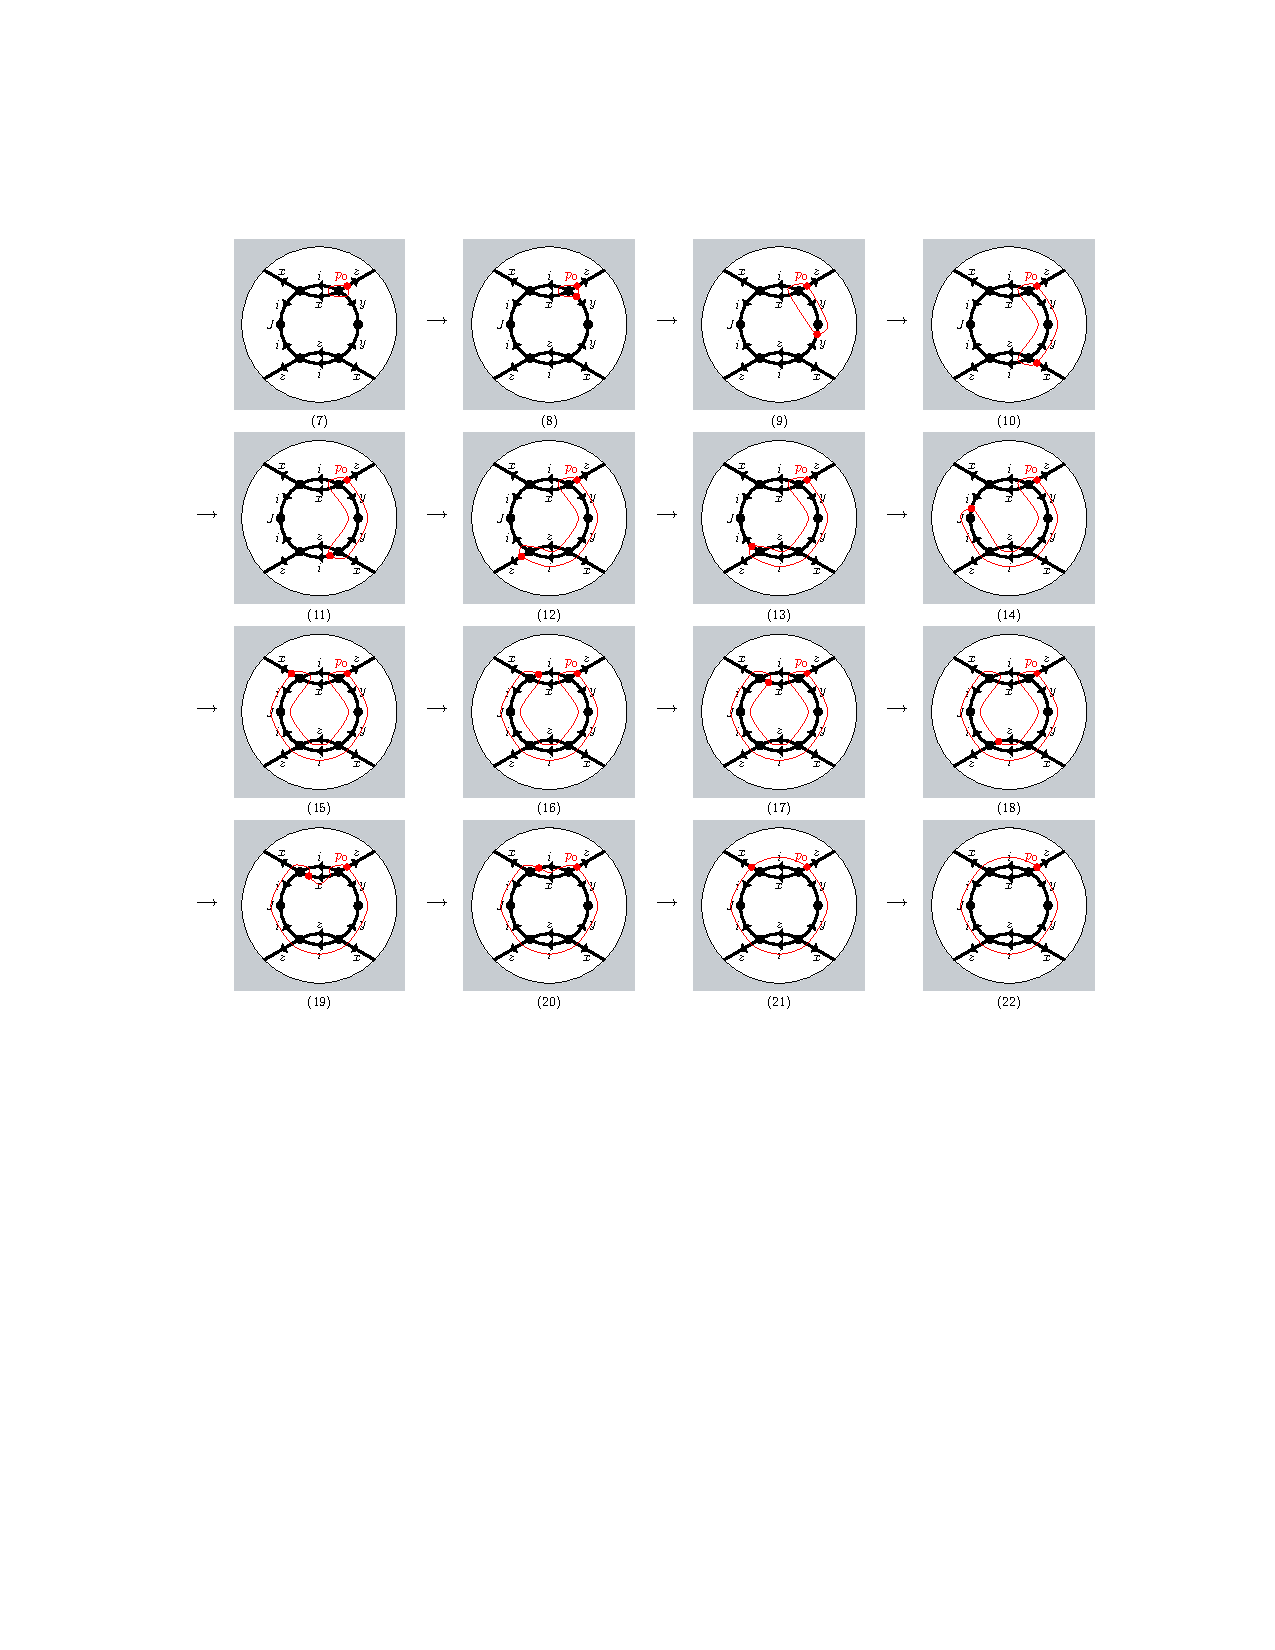
\includegraphics{quant-van-kampen}}

\caption{An instantiation of Algorithm \ref{algorithm:quant-van-kampen} on a group picture for the anticommutation of the qubit Pauli $X$ and $Z$ using the relations $ixyz = 1, y^2 = 1, i^2 = J$. 
Each diagram, together with its associated equation, represents the state of the memory at some step of the algorithm. Equation \eqref{eq:quant-van-kampen-12} is witnessed by the outer picture, and its truth is established by the whole sequence of equations.}

\begin{multicols}{3}
	~\begin{align}
		\label{eq:quant-van-kampen-0}
		ixyz &= 1\\
		zixy &= 1\label{eq:quant-van-kampen-1}\\
		zixy\1 &= 1\label{eq:quant-van-kampen-2}\\
		zixzix &= 1\label{eq:quant-van-kampen-3}\\
		xzixzi &= 1\label{eq:quant-van-kampen-4}
	\end{align}
	~\begin{align}
		xzixzz\1iz &= 1\label{eq:quant-van-kampen-5}\\
		zxzixzz\1i &= 1\label{eq:quant-van-kampen-6}\\
		zxzixzz\1i\1 &= J\label{eq:quant-van-kampen-7}\\
		zxzixzz\1x\1i\1x &= J\label{eq:quant-van-kampen-8}\\
		xzxzixzz\1x\1i\1 &= J\label{eq:quant-van-kampen-8b}
	\end{align}
	~\begin{align}
		i\1xzxzixzz\1x\1 &= J\label{eq:quant-van-kampen-8c}\\
		x\1i\1xzxzixzz\1 &= J\label{eq:quant-van-kampen-9}\\
		i\1xzxzixx\1 &= J\label{eq:quant-van-kampen-10}\\
		xzxzii\1 &= J\label{eq:quant-van-kampen-11}\\
		zxzx &= J\label{eq:quant-van-kampen-12a}\\
		xzxz &= J\label{eq:quant-van-kampen-12}
	\end{align}
\end{multicols}
\end{figure}
\label{fig:quant-van-kampen}
In order to define the algorithm, we set up some terminology:
The \emph{bubble} is the boundary of the expanding subpicture. A \emph{bubble-intersection} is the intersection between the bubble and an edge of the picture. The \emph{pointer} is a (vertex, edge) pair. In our diagrams, we'll draw it as a dot at the bubble-intersection at the edge near the vertex.
To \emph{advance the pointer} is to move the pointer from its current location to the next bubble-intersection clockwise around the bubble. 

We'll work informally with smooth curves. This approach can be rigorized with notions from differential topology---see e.g.\ \cite{guillemin2010differential} for an introduction to the subject. See \cite{slofstra2016tsirelson} for a more careful topological treatment of group pictures. 
Alternatively, one can use graph embeddings where all the vertices lie at integer coordinates and all curves are piecewise linear, and then argue constructively from there.

\begin{algorithm}\label{algorithm:quant-van-kampen}
	
First, pick an edge $e_0$ incident on the boundary of $\m P$. Let $v_0$ be the interior vertex incident to $e_0$. Initialize the bubble so that $v_0$ is the only vertex inside it, and each edge going out of $v_0$ has exactly one bubble-intersection. Initalize the pointer at the bubble-intersection with $e_0$; call this initial point $p_0$. Additionally, initialize variables $w \in \m F(S)$  a word in the generators and $j \in \braket J$ will be some power of $J$. Set $w$ to be the counterclockwise product of the labels of the edges around $v_0$; pick the order so that the rightmost letter corresponds to the lcoation of the pointer. Set $j$ to be label of $v_0$.

Repeat the following until the pointer returns to $p_0$.
Let $(v,e)$ be the location of the pointer. Let $s$ be the group element labeling $e$. Let $v'$ be the other vertex incident on $e$.
\begin{itemize}
	\item If $v'$ is on the boundary of $\m P$, advance the pointer. Additionally, replace $w$ by $sws\1$, canceling an $ss\1$ term that appears. (In the example of Figure \ref{fig:quant-van-kampen}, this happens immediately after states \eqref{eq:quant-van-kampen-0}, \eqref{eq:quant-van-kampen-3}, \eqref{eq:quant-van-kampen-5}, \eqref{eq:quant-van-kampen-8}, \eqref{eq:quant-van-kampen-12a}.)
	\item If $v'$ is not inside the bubble, continuously deform the bubble to contain $v'$.
	Move the pointer to $(v',e)$ and then advance the pointer.

	Additionally, let $r$ be the counterclockwise  product of the edges around $v'$, starting with $e$. Let $l$ be the label of $v'$. Replace $w$ by $wr$, canceling an $ss\1$ term that appears. Replace $j$ by $J^lj$. 
	(In the example of Figure \ref{fig:quant-van-kampen}, this happens immediately after states \eqref{eq:quant-van-kampen-1}, \eqref{eq:quant-van-kampen-2}, \eqref{eq:quant-van-kampen-4}, \eqref{eq:quant-van-kampen-6}, \eqref{eq:quant-van-kampen-7}.)
	\item If $v'$ is inside the bubble, advance the pointer. 

	If the pointer is now on $(v',e)$, continuously deform the bubble to contain $e$ and move the pointer back to the most recently visited intersection which still exists. Additionally, cancel an $ss\1$ term that was already present in $w$, and replace $w$ by $(s')\1 ws'$, where $s'$ is the generator associated with the final location of the pointer. (In the example of Figure \ref{fig:quant-van-kampen}, this happens immediately after states \eqref{eq:quant-van-kampen-9}, \eqref{eq:quant-van-kampen-10}, \eqref{eq:quant-van-kampen-11}.)

	If instead the pointer is not on $(v',e)$, replace $w$ by $sws\1$, canceling an $ss\1$ term that appears. 
	(In the example of Figure \ref{fig:quant-van-kampen}, this happens immediately after states \eqref{eq:quant-van-kampen-8b}, \eqref{eq:quant-van-kampen-8c}.)
\end{itemize}
\end{algorithm}

\begin{lemma}\label{lemma:quant-van-kampen-induction}
	After each iteration of the main loop of Algorithm \ref{algorithm:quant-van-kampen}, all of the following hold:
\begin{enumerate}[(i)]
	\item The equation $w=j$ is true in $G$.
	\item\label{lemma:quant-van-kampen-induction-2} The equation witnessed by the picture whose boundary is the bubble is $w=j$.
	\item\label{lemma:quant-van-kampen-induction-3} On the counter-clockwise arc from $p_0$ to the pointer, each bubble-intersection is a previous location of the pointer.
	\item\label{lemma:quant-van-kampen-induction-4} On the counter-clockwise arc from $p_0$ to the pointer, there is at most one bubble-intersection with each edge of the graph.
	\item The rightmost letter of the word on the left-hand side of the equation is the group element associated with the pointer.
\end{enumerate}
\end{lemma}
\begin{proof}
	\begin{enumerate}[(i)]
		\item The initial equation is true since it is a relation from the group presentation. Each step of the algorithm preserves truth of the equation, since it multiplies the sides of the equation by equal things.
		\item This is true of the intial equation. To see that each step of the algorithm preserves the property, we examine by cases. If the algorithm moves the pointer but not the bubble, then it cyclically permutes the letters on one side of the equation. This is okay, since ``the equation witnessed by a picture'' is only defined up to cyclic permutation.

		If the algorithm moves the bubble by including a new vertex, then the equation witnessed by the bubble changes by replacing the label of one edge at that vertex by the product of the rest of the edge-labels at that vertex.
		This is also how the algorithm changes the equation, multiplying by the relation of the vertex and canceling the $ss\1$ term of the edge to be replaced.

		If the algorithm moves the bubble to include an edge but no vertices, then the equation witnessed by the bubble changes by canceling an $ss\1$ term for that edge. This is also how the algorithm updates the equation.
		\item 
		This is true at the initial step, since the open arc is empty.
		Each time we move the pointer, we move it in the clockwise direction. Whenever we create new bubble-intersections by including a new vertex, we place the pointer at the counter-clockwise-most bubble-intersection at that vertex.
		\item 
		It suffices to check that whenever the pointer is on an edge $e$ with two bubble-intersections, the algorithm immediately moves the bubble so that there are $0$ bubble intersections with that edge.
		Assume inductively that the condition has been true in all the previous steps of the algorithm. We claim that there are no bubble-intersections on the counter-clockwise arc from the current pointer to the other bubble-intersection on edge $e$. 

		First, we must see that no vertex is enclosed by edge $e$ and the arc. 
		By the inductive hypothesis, any edge intersecting this arc does so at most once. By \eqref{lemma:quant-van-kampen-induction-3}, this bubble-intersection is a previous location of the pointer. If this edge were incident on a vertex in the region of interest, then the algorithm would have moved the bubble to enclose that vertex. Therefore, there are no vertices in the region of interest.

		Now suppose some edge $e'$intersects the arc. Since there is no vertex enclosed by the arc and edge $e$, $e'$ must either intersect $e$ or intersect the arc again. The former contradicts planarity of the graph. The latter contradicts the inductive hypothesis.
		\item 
		% This claim is true at the initialization step. To see that the truth of the claim is preserved by each step of the algorithm, we inspect by cases.

		% Whenever we advance the pointer, we conjugate the equation by the generator at the new pointer. This preserves the truth of the claim.

		% When the algorithm moves the bubble to enclose an edge, it cancels the rightmost two generators and then advances the pointer. This preserves truth of the claim.

		% When the algorithm moves the bubble to enclose a vertex, it right-multiplies the equation by a word whose rightmost letter is the label of the next edge to intersect the bubble

		% This covers all cases in which the algorithm either moves the pointer or changes the equations.
		This is proved by casework similar to the proof of \eqref{lemma:quant-van-kampen-induction-2}.
	\end{enumerate}
\end{proof}

\begin{lemma}
The algorithm always terminates. During the runtime, the pointer leaves from each (vertex, edge) pair at most once. When the algorithm terminates, the equation witness by the bubble is the same as the equation witnessed by the picture. 
\end{lemma}
\begin{proof}

	By parts \eqref{lemma:quant-van-kampen-induction-3} and \eqref{lemma:quant-van-kampen-induction-4} of Lemma \ref{lemma:quant-van-kampen-induction}, we have that the pointer visits each (vertex, edge) pair at most once before visiting $p_0$ twice. But the algorithm terminates when it visits $p_0$ for a second time, never getting the chance to leave it a second time. 

	Once it terminates, the whole bubble is comprised of the counterclockwise arc from the pointer to $p_0$, since those are the same point. Then every edge intersecting the bubble does so in at most one place, and every bubble-intersection is a previous location of the pointer. Therefore, the interior of the bubble contains any vertex attached to an edge which has a bubble-intersection. So all of the edges intersecting the bubble are also edges intersecting the boundary of the whole picture. 

	Conversely, we claim that every vertex is contained in the interior of the bubble. This implies that every edge intersecting the boundary of the picture also intersects the bubble.
	 To see the claim, suppose towards a contradiction that there's a vertex outside the bubble. Take a simple (i.e. loop-free) path from that vertex to a vertex in the interior of the bubble. This path intersects the bubble at an edge which does not intersect the boundary of the picture; contradiction. 

	Since the bubble contains the same vertices and intersects the same edges as the picture, they witness the same equation. 

\end{proof}


\subsection{Quantitative stabilizer state bounds}
\label{subsection:quant-stabilizer-state-bounds}

% To finish our collection of tools, we show that if a state is approximately stabilized by the simultaneous action of the Pauli group on two tensor factors, then the state is almost maximally entangled between those factors. This will allow us to deduce self-testing of the provers' state from self-testing of their operators.

To finish our collection of tools, we show that if a state is approximately stabilized by the simultaneous action of an irreducible group representation on two tensor factors, then the state is almost maximally entangled between those factors. This will allow us to deduce self-testing of the provers' state from self-testing of their operators.


% rewrite as being about the standard representation 

% \begin{definition}[Qudit Pauli matrices]\label{definition:qudit-pauli-matrices}
% 	% We define the \emph{qudit Pauli matrices} $X$ and $Z$ as follows. 
% 	Define two matrices over $\C^d$ as follows. $X$ is the matrix for the linear operator acting as $X:\ket a \mapsto \ket{a+1 \pmod d}$. $Z$ is the $p\times p$ matrix for the operator acting as $Z: \ket a \mapsto \w_d^a\ket a$. 
% \end{definition}

% From the qudit Paulis, we define stabilizer operators for the maximally entangled state.
% \begin{definition}
% 	Fix an integer $n\geq 1$. For $i\in [n]$, 
% 	let $\tau(x_i)$ be the operator on $(\C^d)^{\otimes n}$ which acts as $X$ on the $i\th$ tensor factor and and as $I$ on the rest. 
% 	Similarly, 
% 	let $\tau(z_i)$ be the operator on $(\C^d)^{\otimes n}$ which acts as $Z$ on the $i\th$ tensor factor and and as $I$ on the rest. 

% 	For $j\in [2n]$, define operators $S_j$ on $(\C^d)^{\otimes n}\otimes (C^d)^{\otimes n}$ as 
% 	\begin{align}
% 	S_{2k-1} &=\tau(x_k)\otimes \bar{\tau(x_k)},
% 	\\S_{2k} &= \tau(z_k)\otimes \bar{\tau(z_k)}
% 	.
% 	\end{align}
% 	(The complex conjugates here are the reason we chose a basis in Definition \ref{definition:qudit-pauli-matrices}.)
% 	Furthermore, for $\a\in \Z_d^{2n}$, define
% 	\begin{equation}
% 		S_\a = \prod_{i}S_i^{\a_i}.
% 	\end{equation}
% \end{definition}
\begin{lemma}
	% Let $\tau = \tau_1$ be the representation from Definition \ref{def:representations-pauli-group}.
	% The maximally entangled pure state is the uniform combination of the values of $\tau(x)\otimes \bar{\tau (x)}$ $S_\a$, i.e.\
	Let $\tau:\Gamma \to U(\C^d)$ be an irreducible representation with $\Gamma$ a finite group. Then the maximally entangled state can be characterized as a uniform combination of operators from the image of $\tau\otimes \bar{\tau}$. In particular,
% 	The maximally entangled state is the uniform combination of the $S_\a$, i.e.\ 
	\begin{equation}
% 		\proj\epr^{\otimes n} = \frac1{d^{2n}}\sum_{\a\in \Z_d^{2n}}S_\a.
        \proj\epr = \E{g\in \Gamma}\tau(g) \otimes \bar{\tau(g)}.
	\end{equation}
\end{lemma}
\begin{proof}
	We'll show four intermediate equations via simple computations.
	\begin{enumerate}
		\item $\rho_{AB} = \rho_{AB}\dagg$
		\item $\Tr \rho_{AB} = 1$
		\item $\rho_{AB}^2 = \rho_{AB}$
		\item $\Tr_B \rho_{AB}$ is maximally mixed.
	\end{enumerate}
	The first two items assert that $\rho_{AB}$ is a density matrix. The third shows that it is in fact pure. The fourth tells us that the state is maximally entangled across the $A/B$ cut. This characterizes the state.

	Our main trick for the whole proof will be to relabel the index of summation defining $\rho_{AB}$. 
	To prove the first item, we use the relabeling $x\mapsto x\1$. 
	\begin{align*}
		\rho_{AB} 
		&= \E x \tau(x)_A \otimes \bar{\tau(x)}_B
		\\&= \E x \tau(x\1)_A \otimes \bar{\tau(x\1)}_B
		\\&= \E x \tau(x)_A\dagg \otimes \bar{\tau(x)}_B\dagg
		\\&= \left[\E x \tau(x)_A \otimes \bar{\tau(x)}_B\right]\dagg
		\\&= \rho_{AB}\dagg.
	\end{align*}
	(Notice we've used the fact that $\tau(x)$ is unitary; this is one of several parts of the proof that relies on the finiteness of $\Gamma$.) Now define the character $\chi(x):= \Tr \tau(x)$ to compute:
	\begin{align*}
		\Tr \rho_{AB}
		&= \Tr \E x \tau(x)_A \otimes \bar{\tau(x)}_B
		\\&= \E x \chi(x) \bar{\chi(x)}
		\\&= 1.
	\end{align*}
	The final equation is true for the character of any irreducible representation character, and is referred to as the ``second orthogonality relation" in Dummit and Foote \cite{dummit2004abstract}. For the second item,
	\begin{align*}
		\rho_{AB}^2 
		&= \left(\E x \tau(x)_A \otimes \bar{\tau(x)}_B\right)^2
		\\&= \E x\E y \tau(x)_A\tau(y)_A \otimes \bar{\tau(x)}_B\bar{\tau(y)}_B
		\\&= \E x\left[\E y \tau(xy)_A \otimes \bar{\tau(xy)}_B\right]
		\\&= \E x\left[\E y \tau(y)_A \otimes \bar{\tau(y)}_B\right]
	\end{align*}
	In the last line, we used the relabeling $y \mapsto xy$. Continuing, we have
	\begin{align*}
		&= \E x\rho_{AB}
		\\&= \rho_{AB}.
	\end{align*}
	Now define $\rho_A = \Tr_B \rho_{AB}$. Let $y\in \G$ be arbitrary and use the relabeling $x \mapsto yxy\1$:
	\begin{align*}
		\rho_A 
		&= \E x \bar{\chi(x)}\tau(x)
		\\&= \E x \bar{\chi(yxy\1)}\tau(yxy\1)
		\\&= \E x \bar{\chi(x)}\tau(y)\tau(x)\tau(y)\1
		\\&= \tau(y)\left[\E x \bar{\chi(x)}\tau(x)\right]\tau(y)\1
		\\&= \tau(y)\rho_A\tau(y)\1.
	\end{align*}
	So $\rho_A$ commutes with $\tau(y)$ for all $y$. By Schur's lemma (Fact \ref{fact:schur}), $\rho_A$ is a scalar multiple of identity. Since $\Tr\rho_A = 1$, we know that $\rho_A$ is in fact the maximally mixed state. 
	
	Since the maximally entangled state of local dimension $d$ on systems $A$ and $B$ is the unique pure state such that the partial trace over either system gives a maximally mixed state, this concludes our proof. 
\end{proof}
% \begin{proof}
% 	Let $\B\in \Z_d^{2n}$.
% 	From general stabilizer state theory \cite{gottesman1999fault}, it follows that there is a unique one-dimensional subspace, call it $\Span\set{\ket \B}$, such that $\Braket{\B| S_i | \B} = \w_d^{\B_i}$ for all $i$. Furthermore, the $\ket\B$ form an orthonormal basis for $(\C^d)^{\otimes n}\otimes (\C^d)^{\otimes n}$. Now we'll compute the action of the linear operator $\sum_{\a\in \Z_d^{2n}}S_\a$ as
% 	\begin{equation}
% 	\sum_{\a\in \Z_d^{2n}}S_\a\ket \B = d^{2n}\d_{0^{2n},\B}\ket \B,
% 	\end{equation}
% 	which suffices to establish the lemma. First, notice that $\Braket{0^{2n}|S_\a|0^{2n}} = 1$ for any $\a$. Next, suppose that $\B_i \neq 0$. Then we compute
% 	\begin{align}
% 		\sum_{\a\in \Z_d^{2n}}S_\a \ket\B
% 		&=\sum_{l\in \Z_d}\sum_{\a:\a_i = l}S_\a \ket \B
% 		\\&=\sum_{l\in \Z_d}\sum_{\a:\a_i = l}\w_d^{\B_il}\ket \B
% 		\\&=\sum_{\a:\a_i = l}\left(\sum_{l\in \Z_d}(\w_d^{\B_i})^l\right) \ket\B
% 		\\&=0,
% 	\end{align}
% 	where we've used the fact that for $\w$ any $d\th$ root of unity, $\sum_{l\in \Z_d}\w^l = 0$. 
% \end{proof}
\begin{cor}\label{lemma:stabilizer-state}
	Let $\m H_A \cong \m H_B \cong \C^d$. Let $\rho_{ABC}$ be a state on $\m H_A\otimes \m H_B \otimes \m H_C$. Let $\rho_{AB} = \Tr_C\rho_{ABC}$. 

% 	Suppose that for each $\a\in \Z_d^{2n}$, $\drho{\rho_{AB}}{S_\a}I \leq \eta$. 
	Let $\Gamma$ be a finite group. Suppose that for each $g\in \Gamma$, $\drho{\rho_{AB}}{\tau(g)\otimes \bar{\tau(g)}}I \leq \eta$. 

	Then there is a state $\rho_{\text{aux}}$ such that $\norm{\rho_{ABC} - \proj\epr\otimes \rho_\text{aux}}_1 \leq 6\eta^2$.
\end{cor}
\begin{proof}
By linearity, we compute
\begin{align}
	\drho{\rho_{AB}}{\proj \epr}I^2
	&=\drho{\rho_{AB}}{\E{g\in \Gamma}\tau(g)\otimes\bar{\tau(g)}}I^2
	\\&=\E{g \in \Gamma}\drho{\rho_{AB}}{\tau(g)\otimes\bar{\tau(g)}}I^2
	\\& \leq \eta^2.
\end{align}
An application of Lemma \ref{lemma:entanglement-monogamy} completes the proof.
	 
\end{proof}

\subsection{Robust self-testing}\label{subsection:robust-self-testing}

Now we prove a robust self-testing theorem for linear constraint system games. First, we specify precisely what we mean by robust self-testing.

\begin{definition}[Robust self-testing for LCS games]\label{defn: robust-self-testing}
	Let $G$ be an LCS game and $\set{\tilde A_e^{(v)}}, \set{\tilde B_e}, \ket\psi$ be a strategy presented via observables. Let $\d:\R \to \R$ be a continuous function with $\d(0) = 0$. We say that $G$ 
	\emph{self-tests} 
	the strategy with
	\emph{perfect completeness}
	and
	\emph{$\d$-robustness}
	if:
	\begin{itemize}
		\item The strategy $\set{\tilde A_e^{(v)}}, \set{\tilde B_e}, \ket\psi$ wins the game with probability $1$, and
		\item for every strategy $\set{A_e^{(v)}}, \set{B_e}, \rho$ which wins with probability at least $1-\e$, there is a local isometry $V = V_A\otimes V_B$ and auxiliary state $\rho_{\text{aux}}$ such that for every $e,v$ with $H(e,v)\neq 0$,
	\begin{align}
		\label{eq:robustness-condition-state}
		\norm{V\rho V^\dagger - \proj \psi\otimes \rho_{\text{aux}}}_1 &\leq \d(\e),\\
		\drho{V\rho V^\dagger}{V_A A_e^{v}V_A^\dagger\otimes I_A}{(\tilde A_e^{v}\otimes I) \otimes I_B}^2 &\leq \d(\e)\text{, and}\label{eq:robustness-condition-alice}\\
		\drho{V\rho V^\dagger}{I_A\otimes V_BB_eV_B^\dagger}{I_A\otimes (\tilde B_e\otimes I)}^2 &\leq \d(\e).\label{eq:robustness-condition-bob}
	\end{align}

	\end{itemize}
\end{definition}





We restrict our attention only to LCS games with sufficiently nice solution groups.
\begin{definition}\label{definition:group-test}
	Let $\G$ be a finite solution group over $\Z_d$ and $\tau:\G \to U(\C^d)$ an irreducible representation of $\G$ with $\tau(J) = \w_dI$. We say that $\G$ \emph{group-tests $\tau$}  
	if:
	\begin{itemize}
		\item every representation of $\G$ which sends $J \mapsto \w_dI$ is equivalent to $\tau$, and
		\item every irreducible representation of $\G$ sends $J$ to $\w_d^{j}I$ for some $j\in \Z_d$.
	\end{itemize}
\end{definition}
Our second condition may seem artificial. What we really need is the existence of some $\d$ such that if $\s$ is any irreducible not equivalent to $\tau$, then $\norm{\s(J)-\tau(J)}_2 \geq \delta$. This condition gives that to us with $\delta = \Theta(d\1)$.


\begin{theorem}\label{thm:robust-self-testing}
	Let $G$ be an LCS game over $\Z_d$ with vertex set $V$, edge set $E$, and constraints given by  $H:V\times E \to \Z_d$ and $l: V\to \Z_d$. Let $\G$ be the solution group of $G$. Suppose that:
	\begin{enumerate}[(i)]
		\item \label{assumption:bounded-degree}
		 $\abs E \leq \Delta$, $\abs V \leq \Delta$, and
		 each equation has at most $\Delta$ variables with multiplicity, i.e.\ \mbox{$\forall v:\sum_e\abs{H(v,e)} \leq \Delta$},
		\item \label{assumption:small-pictures}there is a canonical form $\can$ such that\footnote{We'll also need a technical assumption that for all $x\in \G$, $\can(Jx) = J\can(x)$ or $\can(Jx) = J^{1-d}\can(x)$.} 
		every equation of the form  $\can(e)e\1 = 1$ for $e\in E$ or $\can(g)\can(gh)\1\can(h) = 1$ for $g,h\in \G$ is witnessed by a $\G$-picture in which 
		 each variable is used at most $\Delta$ times
		 and 
		 each relation is used at most $\Delta$ times,
		\item \label{assumption:w-p-irreps}
		 $\G$ group-tests $\tau: \G \to U(\C^{d^n}) $ in the sense of Definition \ref{definition:group-test}.
% 		\item \label{assumption:pauli-in-image}The image of $\tau$ contains an isomorphic copy of the Pauli group $\m P_d^{\otimes n}$. 
	\end{enumerate}
	Then $G$ self-tests the strategy $\tilde A_e^{(v)} = \tau(e), \tilde B_e = \bar{\tau(e)}, \ket\psi = \ket{\r{EPR}_{d^n}}$
	with perfect completeness and $O(d^2\Delta^{10}\e)$-robustness.

\end{theorem}
The fact that the strategy wins the game with probability $1$ is proven as Proposition \ref{prop: perfect strategy}. The special case of $\e=0$ is the main result of \S \ref{subsection:exact-self-testing}. We remark that although the robustness bound does not seem to depend directly on $n$, typically $\Delta$ does.

The theorem is stated for finite solution groups. Using the stability lemma from \cite{de2017operator}, almost every part of the proof goes through for amenable\footnote{A countable group is \emph{amenable} if it admits a finitely-additive translation-invariant probability measure which is defined on every subset. For a finite group $\G$, we can take this measure as the familiar $\E{x\in \G}$. More exotic examples exist among infinite groups.} groups. However, we crucially use that the length of proofs of group equations is bounded by a constant, which is not true for infinite groups. It seems plausible that this barrier can be overcome; we leave this to future work. To avoid overloading notation, we stated Theorem \ref{thm:robust-self-testing} with sub-optimal bounds. A version of it with tighter, but more notation-involved, bounds is stated and proved in the Appendix as Theorem \ref{thm:robust-self-testing-appendix}.


We break the proof into several lemmas. In the statement of each lemma, we point out which of the assumptions of the main theorem we use. Before we proceed with the proof, we fix some useful notation.  We write $\prod_{i=1}^ng_i$ for the ordered product $g_1g_2\cdots g_n$. 
We write $r_v$ for the relation in $\G$ corresponding to equation $v\in V$, note that this is a word in the generators, say $r_v = s_1s_2\ldots s_n$. We write $\prod_{s\in r_v}f(r_v)$ for the ordered product $f(s_1)f(s_2)\cdots f(s_n)$. 
For $e,e' \in E$, we say $e\sim e'$ if they share an equation, i.e.\ there is some $v$ such that $H(v,e) \neq 0 \neq H(v,e')$. Furthermore, for each edge $e$, we fix a special vertex $v_e$ such that $H(v_e,e)\neq 0$.


\begin{lemma}[Assumption \eqref{assumption:bounded-degree}]\label{lemma:Bs-are-approximate-conjugate-operator-solution}
	$\set{B_e}$ is an ``approximate conjugate operator solution'' in the following sense:
	\begin{align}
	\label{eq:Bs-approximately-satisfy-constraints}
		\sum_v \drho{\rho}{
		\prod_{e\in r_v} I_A\otimes B_e}{\w_d^{-l(v)}I_{AB}} 
		&\leq 4\Delta^2\sqrt\e.
		\\
	\label{eq:Bs-approximately-commute}
		\sum_{e,e':e\sim e'} \drho{\rho}{I_A\otimes [B_e,B_{e'}]}{I_{AB}}
		&\leq 4\Delta^3\sqrt\e
		.\
	\end{align}

	Furthermore, we have similar inequalities for Alice, 
	\begin{align}
	\label{eq:As-approximately-satisfy-constraints}
		\sum_v\drho{\rho}{\prod_{e\in r_v}A_e^{(v_e)}\otimes I_B}{\w_d^{l(v)} I_{AB}}
		&\leq 8\Delta^2\sqrt{\e},
		\\
	\label{eq:As-approximately-commute}
		\sum_{e,e':e\sim e'} \drho{\rho}{\left[A_e^{(v_e)},A_{e'}^{(v_{e'})}\right]\otimes I_B}{I_{AB}}
		&\leq 4\Delta^3\sqrt\e
		.
	\end{align}
	Finally, these ``solutions'' are consistent in the sense that
	\begin{equation}
	\label{eq:As-and-Bs-approximately-consistent}
		\sum_e \drho{\rho}{A_e^{(v_e)}\otimes I_B}{I_A\otimes B_e^\dagger}
		 \leq 2 \Delta^2\sqrt\e.
	\end{equation}
\end{lemma}
Equation \eqref{eq:Bs-approximately-satisfy-constraints} says that Bob's operators approximately satisfy the group equations induced by the constraints. Equation \eqref{eq:Bs-approximately-commute} says that Bob's operators approximately commute whenever they share an equation.
\begin{proof}
	Recalling the consistency criterion \eqref{eq:approximate-win-criterion-con}, we have 
	\begin{align}
		\frac14\E{e,v}\drho{\rho}{A_e^{(v)}\otimes B_e}{I}^2 \leq \e.
	\end{align}
	An application of Cauchy-Schwarz 
	and then Lemma \ref{lemma:state-dependent-distance}\eqref{item:state-dependent-distance-inverse} 
	gives
	\begin{align}
		\sum_{e,v:H(v,e)\neq 0} \drho{\rho}{A_e^{(v)}\otimes B_e}{I} 
		&\leq 2 \abs E \abs V\sqrt\e \nonumber
		\\
		\sum_{e,v:H(v,e)\neq 0} \drho{\rho}{A_e^{(v)}\otimes I_B}{I_A\otimes B_e^\dagger}
		 &\leq 2 \Delta^2\sqrt\e. \label{eq:Bs-are-approximate-operator-solution-1}
	\end{align}
	Inequality \eqref{eq:As-and-Bs-approximately-consistent} can be obtained from inequality \eqref{eq:Bs-are-approximate-operator-solution-1} by dropping some (nonnegative) terms from the left-hand side.
	Similarly, we extract the following from the constraint satisfaction criterion \eqref{eq:approximate-win-criterion-sat}.
	\begin{align}
	\label{eq:Bs-are-approximate-operator-solution-2}
		\sum_v \drho{\rho}{
		\prod_{e\in r_v} A_e^{(v)} \otimes I}{\w_d^{l(v)}I}
		\leq 2 \sqrt \e \abs V.
	\end{align}
	Applying a triangle inequality and taking inverses (see \ref{lemma:state-dependent-distance}\ref{item:state-dependent-distance-triangle},\ref{item:state-dependent-distance-chaining}) to the previous two equations yields
	\begin{align}
		\sum_v \drho{\rho}{
		\prod_{e\in r_v} I_A\otimes B_e}{\w_d^{-l(v)}I_{AB}} 
		&\leq 2\Delta^2\sqrt\e +2 \abs V\sqrt\e
		,
	\end{align}
	establishing Equation \eqref{eq:Bs-approximately-satisfy-constraints}. 
	We use the same strategy for the commutators. First, note that Alice's operators commute exactly, i.e.\
	\begin{equation}
	\label{eq:Bs-are-approximate-operator-solution-3}
	\drho{\rho}{\left[A_e^{(v)}, A_{e'}^{(v)}\right]\otimes I_B} {I_{AB}} 
	= 0\text{ if }e\sim e'.
	\end{equation}
	Then we can chain triangle inequalities to deduce a bound on the magnitude of Bob's commutators:
	\begin{equation}
	\drho{\rho}{I_A\otimes \left[B_e,B_{e'}\right]}{I}
	\leq 
	2\drho{\rho}{A_e^{(v)}\otimes B_e}{I_{AB}}
	+2\drho{\rho}{A_{e'}^{(v)}\otimes B_{e'}}{I_{AB}}.
	\end{equation}
	Since we know the right-hand-side to be small on average, we sum over all equations and then apply Equation \eqref{eq:Bs-are-approximate-operator-solution-1}:
	\begin{align}
	\sum_{\substack{e,e'\\e\sim e'}}\drho{\rho}{I_A\otimes \left[B_e,B_{e'}\right]}{I}
	&\leq
	2\Delta \sum_{\substack{e,v\\H(v,e)\neq 0}}
	\drho\rho{A_e^{(v)}\otimes B_e}{I_{AB}}	
	\\
	&\leq 4\Delta^3\sqrt \e
	,
	\end{align}
	establishing Equation \eqref{eq:Bs-approximately-commute}.
	In the first line, we used that each equation has at most $\Delta$ variables. In the second line, we applied inequality \eqref{eq:Bs-are-approximate-operator-solution-1}.

	By reasoning on the $B$ system, we proved 
	Equations \eqref{eq:Bs-approximately-satisfy-constraints}, \eqref{eq:Bs-approximately-commute}
	from Equations \eqref{eq:Bs-are-approximate-operator-solution-1}, 
	\eqref{eq:Bs-are-approximate-operator-solution-2},
	\eqref{eq:Bs-are-approximate-operator-solution-3}. The same arguments on the $A$ system prove Equations \eqref{eq:As-approximately-satisfy-constraints}, \eqref{eq:As-approximately-commute}
	from Equations
	\eqref{eq:Bs-approximately-satisfy-constraints},
	\eqref{eq:Bs-approximately-commute},
	\eqref{eq:Bs-are-approximate-operator-solution-1}.

\end{proof}

In order to apply the stability lemma of \S \ref{subsection:stability-lemma}, we need to construct a function from the solution group to the group of unitaries. 
We already have functions defined on the generators: those which send $e\mapsto A_e^{(v_e)}$ and $e\mapsto B_e$. We would like to say ``extend $f_A$ and $f_B$ to all of $\G$ by multiplication''. However, these functions are not quite homomorphisms, so different choices of how to ``extend by multiplication'' define different functions. We'll use our canonical form $\can$ to make that choice in a consistent way. 
\begin{definition}
\label{def:4.19}
	%For each edge $e$, pick a vertex $v_e$ such that $H(v_e,e)\neq 0$. 
	Define $f_A:\G\to U(\m H_A)$ and $f_B:\G\to U(\m H_B)$ by
	 % setting $f_A(J) = \w_dI, f_B(J) = \w_d\1I$, $f_A(e) = A_e^{(v_e)}, f_B(e)$ and
	\begin{align}
		f_A(g) = \begin{cases}
			\w_d I, &\text{ if }g=J\\
			A_e^{(v_e)}, &\text{ if }\can(g)=e\\
			\prod_{s\in \can(g)} f_A(s), &\text{ otherwise,}
		\end{cases}
		\\
		f_B(g) = \begin{cases}
			\w_d\1 I, &\text{ if }g=J\\
			B_e, &\text{ if }\can(g)=e\\
			\prod_{s\in \can(g)} f_B(s), &\text{ otherwise.}
		\end{cases}
	\end{align}
\end{definition}
Notice that we may have generators $e$ of the group for which $f_B(e) \neq B_e$. For example, in our canonical form for the Magic Square game defined in section \ref{sec:specific-games}, we'll have $\can(e_3) = e_1\1e_2\1$. If the equation $B_1B_2B_3 = I$ does not hold exactly, we have that $f(e_3) = B_1\1B_2\1 \neq B_3$. However, we do want $f(e_3)$ to be close to $B_3$. This is the content of the first item of the next lemma.

\begin{lemma}[Assumption \eqref{assumption:small-pictures}]\label{lemma:canonical-form-implies-stability}
	% Let $R$ be the set of relations (both commutation and constraint) in the presentation for $\G$, and let $w,f_A,f_B$ be as in the statement of Theorem \ref{thm:robust-self-testing}.
	Suppose that $\set{A_e^{(v_e)}}$ and $\set{B_e}$ $\eta$-satisfy the relations from $R$ in the sense that
	\begin{equation}
	\label{lemma:canonical-form-implies-stability-1}
		%\sum_{r\in R} \drho{\rho}{\prod_{e\in r}{A_e^{(v_e)}\otimes I_B}}{I_{AB}} \leq \eta\text{, and }
		%\sum_{r\in R} \drho{\rho}{I_A\otimes \prod_{e\in r}{B_e} }{I_{AB}} \leq \eta.
		\sum_v\drho{\rho}{\prod_{e\in r_v}A_e^{(v_e)}\otimes I_B}{\w_d^{l(v)} I_{AB}} \eta\text{, and }
		\sum_{e,e':e\sim e'} \drho{\rho}{\left[A_e^{(v_e)},A_{e'}^{(v_{e'})}\right]\otimes I_B}{I_{AB}} \leq \eta
	\end{equation}
	And similarly for $B$ we have 
	\begin{equation}
	\label{lemma:canonical-form-implies-stability-1-B}
	\sum_v \drho{\rho}{
		\prod_{e\in r_v} I_A\otimes B_e}{\w_d^{-l(v)}I_{AB}} \leq \eta\text{, and }
		\sum_{e,e':e\sim e'} \drho{\rho}{I_A\otimes [B_e,B_{e'}]}{I_{AB}}
	\end{equation}
	 Furthermore, suppose that $\set{A_e^{(v_e)}}$ and $\set{B_e}$ are $\eta$-consistent, i.e.\ 
	 \begin{equation}
	 \label{lemma:canonical-form-implies-stability-2}
	 	\sum_e \drho{\rho}{A_e^{(v_e)}\otimes B_e}{I_{AB}} \leq \eta.
	 \end{equation}
	  Then 
	  \begin{enumerate}[(1)]
	  	\item 
	  for all $e\in E$, the operators $f_A(e)$ and $f_B(e)$ are close to the operators used by Alice and Bob, i.e.\ 
	  \begin{align}
	  \label{eq:canonical-form-implies-stability-conclusion-1}
	  	\drho{\rho}{f_A(e)\otimes I_B}{ A_e^{(v_e)}\otimes I_B } &\leq 8\Delta \eta,
	  	\\
	  	\drho{\rho}{I_A \otimes f_B(e)}{ I_A \otimes B_e} &\leq 8\Delta\eta. 
	  \end{align}
	\item \label{item:canonical-form-implies-stability}$f_A$ and $f_B$ are suitable for application of the stability lemma \ref{lemma:vidick-gowers-hatami}, i.e.\ for all $x,y\in \G$, 
	\begin{align}
	\label{eq:canonical-form-implies-stability}
		\drho\rho{f_A(x)f_A(yx)\1f_A(y)\otimes I_B}{I_{AB}} &\leq 64\Delta^2\eta,
		\\
		\drho\rho{I_A\otimes f_B(x)f_B(yx)\1f_B(y)}{I_{AB}}&\leq 64\Delta^2\eta.
	\end{align}
	\item \label{item:canonical-form-implies-consistency}$f_A$ and $f_B$ are consistent, i.e.\  for all $x\in \G$,
	\begin{equation}
	\label{eq:canonical-form-implies-consistency}
		\drho\rho{f_A(x)\otimes f_B(x)}{I_{AB}} \leq 4\Delta\eta.
	\end{equation}
  \end{enumerate}

\end{lemma}
For our purposes, it would suffice to prove items \eqref{item:canonical-form-implies-stability} and \eqref{item:canonical-form-implies-consistency} on average over $g$ and $h$. This may make the upper bound smaller, but the authors presently know of no families of groups for which this improvement is better than a constant factor. 
\begin{proof}
	By the quantitative van Kampen lemma (Lemma \ref{lem:quant-van-kampen}), any identity of the form $\can(e)e\1 = 1$ has a proof using at most $2\Delta$ conjugations by each generator and at most $\Delta$ right-multiplications by each relation. In this proof, we replace each instance of a generator $e$ with the corresponding Bob operator $I\otimes B_{e}$, and replace the equality by a bound of the $\drho\rho\cdot\cdot$-distance between the two sides. By at most $2\Delta$ applications of Lemma \ref{lemma:state-dependent-distance}(\ref{item:state-dependent-distance-right-multiplication}) and at most $\Delta$ applications of Lemma \ref{lemma:state-dependent-distance}(\ref{item:state-dependent-distance-conjugation}), we get the bound on the $\drho\rho\cdot\cdot$-distance stated in Equation \eqref{eq:canonical-form-implies-stability-conclusion-1}. Repeating the same proof for identities of the form $\can(x)\can(yx)\1\can(y)$ but now starting from the $f_B(e)$ instead of the $B_e$ gives the second part of Equation \eqref{eq:canonical-form-implies-stability}. The same argument with the tensor factors reversed gives the first part.

	Finally, we obtain, using Lemma \ref{lemma:state-dependent-distance}\eqref{item:state-dependent-distance-chaining},
	\begin{align}
		\drho\rho{f_A(g)\otimes f_B(g)}{I_{AB}} 
		&= \drho{\rho}{\prod_{e\in \can(g)}{ A_e^{(v_e)}\otimes B_e}}{I_{AB}}
		\\&\leq \sum_{e\in \can(g)} 
		\drho\rho{A_e^{(v_e)}\otimes B_e}{I_{AB}}.
	\end{align}
	Each word in the canonical form must use at most $\Delta$ occurences of each generator, since all such occurences appear in a group picture with the word on the boundary. So we have
	\begin{align}
		\sum_{e\in \can(g)} 
		\drho\rho{A_e^{(v_e)}\otimes B_e}{I_{AB}}
		&\leq \Delta\sum_{e\in E} 
		\drho\rho{A_e^{(v_e)}\otimes B_e}{I_{AB}}
		\\&\leq \Delta \eta.
	\end{align}
\end{proof}

\begin{lemma}[Assumption \eqref{assumption:w-p-irreps}]
\label{lemma:fixing-the-J}
	Let $f:\G\to \m L(\m H)$ be such that $f(1)$ is a projection and $f(Jx) = \w_df(x)$ for all $x$. 
	Let $\s: \G \to U(\m H)$ be a representation. Let $\rho$ be a state on $\m H$. Finally, suppose $\E{x}\drho\rho{f(x)}{\s(x)} \leq \eta$. 

	Then there is a projection $P$ such 
	that $P$ commutes with $\s(x)$ for each $x$, $P\s(J)P = \w_dP$, and $\drho\rho PI \leq d \eta$. The same holds if we replace $\w_d$ by $\w_d\1$.\footnote{Indeed, we could replace $\w_d$ by $\w_d^k$ for any $k$ coprime to $d$.}
\end{lemma}
\begin{proof}
	Decompose $\s = \bigoplus_i \s_i$ as a sum of irreducibles. 
	For each $j \in \Z_d$, let $P_j$ be the projection onto the $\w_d^j$-eigenspace of $\s(J)$.
	Notice that these decompositions are compatible in the following sense: for each $i,j$, the map $x\mapsto P_j\s_i(x)P_j$ is either the all $0$-map or it is a representation on the range of $P_j$ sending $J$ to $\w_d^jI$. It follows that $x\mapsto P_1 \s(x)P_1$ is an operator solution. Now we compute, using inequality \ref{lemma:convex-inequality-hard},
	\begin{align}
	\frac12\drho\rho PI^2 
	&= 1 - \Re\Tr_\rho P
	\\
	\frac12\drho\rho PI^2
	&\leq \frac14d^2\left[
		1 - \Re\Tr_\rho\w_d\1\s(J)
	\right]
	\\
	\frac12\drho\rho PI^2
	&\leq \frac12\left(\frac d2\drho\rho{\s(J)}{\w_dI}\right)^2
	\\
	\drho\rho PI
	&\leq \frac d2\drho\rho{\s(J)}{\w_dI}.
	\end{align}
	The lemma will be established if we can show $\drho\rho{\s(J)}{\w_dI} \leq 2 \eta$. We first use the fact that expectation is invariant to multiplication by $J$.
	\begin{align}
		\E{x}\drho\rho{f(x)}{\s(x}
		&=\E{x}\drho\rho{f(Jx)}{\s(Jx)}
		\\&=
		\E{x}\drho\rho{\w_df(x)}{\s(J)\s(x)}
		\\&=
		\E{x}\drho\rho{f(x)}{w_d\1\s(J)\s(x)}
	\end{align}
	Next we use the triangle inequality and the unitarity of $\s(x)$. 
	\begin{align}
		\E{x}\drho\rho{\s(x)}{\w_d\1\s(J)\s(x)}
		&\leq 
		\E{x}\drho\rho{f(x)}{\s(x)}
		\E{x}\drho\rho{f(x)}{\w_d\1\s(J)\s(x)}
		\\
		\E{x}\drho\rho{\s(x)}{\w_d\1\s(J)\s(x)}
		&\leq2\eta. 
		\\
		\E{x}\drho\rho{\s(J)}{\w_dI}
		&\leq2\eta. 
	\end{align}
	Notice that the argument of the expectation on the left-hand side does not depend on $x$, so we have 
	\mbox{$\drho\rho{\s(J)}{\w_dI} \leq 2\eta$} unconditionally.
\end{proof}




\begin{proof}[Proof of Theorem \ref{thm:robust-self-testing}]
	By Lemma \ref{lemma:Bs-are-approximate-conjugate-operator-solution}, $f_A$ and $f_B$ each satisfy conditions \eqref{lemma:canonical-form-implies-stability-1}, \eqref{lemma:canonical-form-implies-stability-1-B} and \eqref{lemma:canonical-form-implies-stability-2} 
	with $\eta_1 = 2^4\Delta^3\sqrt \e$. By Lemma \ref{lemma:canonical-form-implies-stability}, $f_A$ and $f_B$ each satisfy the condition of the stability lemma \ref{lemma:vidick-gowers-hatami} with $\eta_2 =2^{10}\Delta^5\sqrt\e$. Applying the stability lemma, we get representations $\s_A,\s_B$ and isometries $W_A,W_B$ such that 
	\begin{align}
	\label{eq:fa-close-to-something}
		\E{x} \drho{\rho}{f_A(x)\otimes I_B}{ W_A^\dagger \s_A(x)W_A\otimes I_B} &\leq \eta_2\text{, and} \\
		\E{x} \drho{\rho}{I_A\otimes f_B(x)}{ I_A \otimes  W_B^\dagger \s_B(x)W_B} &\leq \eta_2. 
	\end{align}
	Recall that $f_A(J) = \w_d$ and $f_B(J) = \w_d\1$. Note that furthermore 
	\begin{equation}
		f_A(Jx) = \w_df_A(x)\text{ and } f_B(Jx) = \w_d\1f_B(x)\text{ for any }x\in\G.
	\end{equation}
	Now we apply Lemma \ref{lemma:fixing-the-J} with $\s=\s_A,\s_B$, $f(x) = W_Af_A(x)W_A^\dagger, W_Bf_B(x)W_B^\dagger$ on the states $(W_A\otimes I_B)\rho (W_A^\dagger \otimes I_B)$,$(I_A\otimes W_B)\rho (I_A\otimes W_B^\dagger)$, respectively. Let $P_A$ and $P_B$ be the resulting projectors. One can check that $x \mapsto P_A\s_A(x)P_A$ is an operator solution, while  $x \mapsto P_B\s_B(x)P_B$ is a conjugate operator solution. By assumption \eqref{assumption:w-p-irreps}, we can apply Lemma \ref{lem:unique-operator-solution} to get isometries ${\tilde W}_A, {\tilde W}_B$ such that
	\begin{align} 
	\label{eq:tau-construction-by-isometry}
	{\tilde W}_AP_A\s_A(x)P_A{\tilde W}_A^\dagger &= \tau(x)\otimes I\text{, and }
	\\
	{\tilde W}_BP_B\s_B(x)P_B{\tilde W}_B^\dagger &= \bar{\tau(x)}\otimes I.
	\end{align}

	% Now we chain many equations.
	Let $V_A = \tilde W_AW_A,V_B = \tilde W_BW_B, V = V_A\otimes V_B$. We compute:
	\begin{align}
		\eta_2 
		&\geq
		\E{x} \drho{(W_A\otimes I)\rho (W_A^\dagger\otimes I)}{W_Af_A(x)W_A^\dagger\s_A(x)^\dagger\otimes I_B}{I_{AB}}
		&& \text{derived from Equation \eqref{eq:fa-close-to-something}}
		\\
		(d+1)\eta_2
		&\geq
		\E{x} \drho{(W_A\otimes I)\rho (W_A^\dagger\otimes I)}{W_Af_A(x)W_A^\dagger\s_A(x)^\dagger P_A\otimes I_B}{I_{AB}}
		&& \text{right-multiply }P_A
		\\&=
		\E{x} \drho{(W_A\otimes I)\rho (W_A^\dagger\otimes I)}{W_Af(x)W_A^\dagger P_A\s_A(x)P_A\otimes I_B}{I_{AB}}
		&& \text{commute }P_A\text{ past }\s(x)
		\\&=
		\E{x} \drho{V\rho V^\dagger}{V_Af_A(x)W_A^\dagger(\tilde W_A^\dagger\tilde W_A) P_A\s_A(x)^\dagger P_A\tilde W_A^\dagger\otimes V_BV_B^\dagger}{\tilde W_A W_A \otimes V_BV_B\dagg}
		&& \text{conjugate by } \tilde W_A\otimes V_B
		\\&=
		\E{x} \drho{V\rho V^\dagger}{V_Af_A(x)W_A^\dagger(\tilde W_A^\dagger\tilde W_A) P_A\s_A(x)^\dagger P_A\tilde W_A^\dagger\otimes I_B}{I_{AB}}
		&& \text{apply Lemma \ref{lemma:state-dependent-distance}\eqref{item:state-dependent-distance-projection-is-identity} twice } 
		\\&=
		\E{x} \drho{V\rho V^\dagger}{V_Af_A(x)V_A^\dagger\otimes I_B}{\tilde W_A P_A\s_A(x) P_A\tilde W_A^\dagger\otimes I_B}
		&& \text{apply Lemma \ref{lemma:state-dependent-distance}\eqref{item:state-dependent-distance-inverse}}
		\\&=
		\E{x} \drho{V\rho V^\dagger}{V_Af_A(x)V_A^\dagger\otimes I_B}{(\tau(x) \otimes I) \otimes I_B}
		&& \text{apply Equation \eqref{eq:tau-construction-by-isometry}.}
	\end{align}
	The same proof works for the $B$ objects, yielding
	\begin{equation}
	\label{eq:robust-self-testing-proof-2}
		\E{x} \drho{V\rho V^\dagger}{I_A \otimes V_Bf_B(x)V_B^\dagger}{I_A \otimes (\bar{\tau(x)} \otimes I)}
		\leq (d+1)\eta_2.
	\end{equation}
	Recalling equation \eqref{eq:canonical-form-implies-consistency} and taking an expectation, we have
	\begin{align}
	\label{eq:robust-self-testing-proof-1}
		4\Delta\eta_1 
		&\geq
		\E{x}\drho{\rho}{f_A(x)\otimes f_B(x)}{I_{AB}}
		\\&=
		\E{x}\drho{V\rho V\dagg}{V_Af_A(x) V_A\dagg\otimes V_Bf_B(x) V_B\dagg}{I_{AB}}
		\\&=
		\E{x}\drho{V\rho V\dagg}{V_Af_A(x) V_A\dagg\otimes I_B}{I_A\otimes V_Bf_B(x)\dagg V_B\dagg}.
	\end{align}
	Weakening the previous inequality for convenience, we have
	\begin{equation}
		\E{x}\drho{V\rho V\dagg}{V_Af_A(x) V_A\dagg\otimes I_B}{I_A\otimes V_Bf_B(x)\dagg V_B\dagg}.\leq \eta_2.
	\end{equation}
	Applying three triangle inequalities gives us
	\begin{equation}
		\label{eq:robust-self-testing-proof-3}
	 	\E x \drho{V\rho V^\dagger}{(\tau(x)\otimes I)_A\otimes (\bar{\tau(x)}\otimes I)_B}{I_{AB}} 
		\leq 3d\eta_2
	 \end{equation}
	 which says that $(\tau(x)\otimes I)_A \otimes (\bar{\tau(x)}\otimes I)_B$ approximately stabilizes $V\rho V^\dagger$ on average. Now we see that a similar bound holds pointwise. We use a change of variable and the homomorphism property of $\tau$; this is the same technique used in the proof of Lemma \ref{lemma:fixing-the-J}.
	\begin{align}
		\E x \drho{V\rho V^\dagger}{(\tau(x)\otimes I)\otimes (\bar{\tau(x)}\otimes I)}{I} 
		&\leq 3d\eta_2
		\\
		\E x \drho{V\rho V^\dagger}{(\tau(yx)\otimes I)\otimes (\bar{\tau(yx)}\otimes I)}{I} 
		&\leq 3d\eta_2
		\\
		\label{eq:robust-self-testing-proof-4}
		\E x \drho{V\rho V^\dagger}{(\tau(y)\tau(x)\otimes I)\otimes (\bar{\tau(y)\tau(x)}\otimes I)}{I} 
		&\leq 3d\eta_2
		\\
		\label{eq:robust-self-testing-proof-5}
		\E x \drho{V\rho V^\dagger}{(\tau(y)\otimes I)\otimes (\bar{\tau(y)}\otimes I)}{I} 
		&\leq 6d\eta_2.
	\end{align}
	The final equation follows from right-multiplying the previous equation by the inverse of Equation \eqref{eq:robust-self-testing-proof-3}. Since the expression has no $x$ dependence, we can drop the average and draw the same conclusion pointwise.

	Now we use the finiteness of the group and apply Corollary \ref{lemma:stabilizer-state}.  We trace out irrelevant subsystems and then apply the conclusion of that lemma:
	\begin{align}
		\forall y\drho{V\rho V^\dagger}{(\tau(y)_{A_1}\otimes I_{A_2})\otimes (\bar{\tau(y)}_{B_1}\otimes I_{B_2})}{I} 
		&\leq 6d\eta_2,
		\\
	\Rightarrow	\,\,\,\,\forall y\drho{\Tr_{A_2B_2}V\rho V^\dagger}{\tau(y)_{A_1}\otimes \bar{\tau(y)}_{B_1}}{I} 
		&\leq 6d\eta_2,
		\\
		\Rightarrow \,\,\,\, \norm{\Tr_{A_2B_2}V\rho V^\dagger - \proj\epr^{\otimes n}\otimes \rho_\text{aux}}_1
		&\leq 6^3(d\eta_2)^2, \,\,\,\,\,\,\,\text{by Corollary \ref{lemma:stabilizer-state}}.
	\end{align}
	This establishes the robustness condition \eqref{eq:robustness-condition-state} with $\d(\e) = O(d^2\eta_2^2) = O(d^2\Delta^{10}\e)$.

	Next, we show the other robustness conditions. It'll suffice to find that $f$ is close to $\tau$ pointwise. 
	Equations \eqref{eq:robust-self-testing-proof-2}, \eqref{eq:robust-self-testing-proof-1} with a triangle inequality give
	\begin{align}
		\E{x}&\drho{V\rho V^\dagger} {V_Af_A(x)V_A^\dagger\otimes (\bar{\tau(x)} \otimes I)_B}{I}\leq 2d\eta_2\text{, and}
		\\
		\E{x}&\drho{V\rho V^\dagger} {(\tau(x) \otimes I)_A\otimes V_Bf_B(x)V_B^\dagger}{I} \leq 2d\eta_2.
	\end{align}
	From here, we argue only on the $A$ side. The argument for the $B$ side is analogous. Applying a change of variable and then multiplying gives
	\begin{align}
		\E{x}\drho{V\rho V^\dagger}{V_Af_A(ex)V_A^\dagger\otimes (\bar{\tau(ex)} \otimes I)}{I} &\leq 2d\eta_2,
		\\
		\E{x}\drho{V\rho V^\dagger}{V_Af_A(ex)f_A(x)^\dagger V_A^\dagger\otimes (\bar{\tau(e)} \otimes I)}{I} &\leq 4d\eta_2.
	\end{align}
	By Equation \eqref{eq:canonical-form-implies-stability},
	\begin{equation}
	\drho{V\rho V^\dagger}{V_Af_A(ex)f_A(x)^\dagger V_A^\dagger\otimes I_B}{V_Af_A(e) V_A^\dagger\otimes I_B} \leq \eta_2.
	\end{equation}
	Using this, Equation \eqref{eq:robust-self-testing-proof-5}, and two triangle inequalities gives
	\begin{equation}
		\drho{V\rho V^\dagger}{V_Af_A(e)V_A^\dagger\otimes I_A}{(\tau(e)\otimes I) \otimes I_B}
		\leq 11d\eta_2.
	\end{equation}
	From the conclusion of Lemma \ref{lemma:canonical-form-implies-stability}, we know that $f_A(e)$ is $\eta_2$-close to $A_e^{(v_e)}$. One more triangle inequality establishes robustness conditions \eqref{eq:robustness-condition-alice}, \eqref{eq:robustness-condition-bob} with $\d = O(d^2\eta_2^2) = O(d^2\Delta^{10}\e)$.


\end{proof}